\section{Dynamic Penalty Optimization}\label{dyn_opt}

%IV.	Dynamic Optimization
%	a.	Gradient Descent w/ Backtracking Search
%		i. boundary conditions clean up
%	b.	Dealing with Fractional Results

\pacora's penalty optimization algorithm dynamically decides resource allocations. The algorithm can be run periodically, when applications start or stop, when an application changes faces or when the system changes operating scenarios.  One of the advantages of convex optimization is that it enables fast, incremental solutions.  As a result the algorithm could terminate earlier to decrease overhead and still be moving towards an optimal solution as it runs.  However we found in our implementation that the algorithm was fast enough to run to completion every time. 

Convex optimization is simplest when it is unconstrained, and so we reformulated \pacora's construction to be unconstrained.
Extending the response time model functions to all of $\Re^n$
moves the requirement that allocations must be positive into the objective function,
and introducing Application 0 for slack resources turns the affine inequalities into equalities:
\begin{eqnarray*}
& \makebox[1in][r]{Minimize}   & \sum_{p\in P} {\pi_p(\tau_p(a_{p,1}\ldots a_{p,n}))}  \\
& \makebox[1in][r]{Subject to} & \sum_{p\in P} a_{p,r} = A_r, r = 1,\ldots n           \\
\end{eqnarray*}

The only remaining constraints are those on the $a_{p,r}$.
These can be removed by letting the $a_{p,r}$ be unbounded above for $p \neq 0$
and changing the domain of $\tau_0$  to be the whole resource allocation matrix.
The definition of $\tau_0$ might take the form
\begin{eqnarray*}
\tau_0 &=& \sum_r \Delta_r \sum_{p \neq 0} a_{p,r}     \\
       &=& \sum_r \Delta_r (A_r - a_{0,r})
\end{eqnarray*}
where $\Delta_r$ is the (constant) power dissipation of one unit of resource $r$.
However,if any of the allocations $a_{0,r}$ turns out to be negative then $\tau_0$  should instead return the value $+\infty$.
This modification of the objective function transforms the resource allocation problem
to unconstrained convex optimization.  


The penalty optimization algorithm used in \pacora is gradient descent via backtracking line search along the negative gradient direction \cite{BoVa}.
This algorithm rejects and refines any step that yields insufficient relative improvement in the objective function,
so infinite values from infeasible allocations will automatically be avoided by the search.
The negative gradient $-\nabla\pi$ of the overall objective function $\pi$
with respect to the resource allocations $a$
is computed analytically from the response time models and penalty functions.
When a component of this overall gradient is negative,
it means the penalty will be reduced by increasing the associated allocation if possible.
The gradient search at the boundaries of the feasible region
must ignore components that lead in infeasible directions;
these can be detected by noting whether for some $p$ and $r$, $a_{p,r} = 0$ with $(-\nabla\pi)_{p,r} > 0$.
In such cases, the associated step component is set to zero.

We added an additional optimization to move along boundaries more rapidly in the scenario when a completely allocated resource had a large gradient.  We scale all the allocations of that resource type down to satisfy resource constraint while leaving the allocations of other resources untouched.

The rate of convergence of gradient descent depends on how well the sublevel sets of the objective function
are conditioned (basically, how ``spherical'' they are).
Conditioning will improve if resource allocation units are scaled to make their relative effects on $t$ similar.
For example, when compared with processor allocation units,
memory allocation units of 4MB are probably a better choice than 4 KB.
In addition, penalty function slopes should not differ by more than perhaps two orders of magnitude. If these measures prove insufficient, stronger preconditioners can be used. In our implementation, we condition all resource allocations to be in the range of 0-50.


\begin{figure}[!t]
	\begin{center}	
		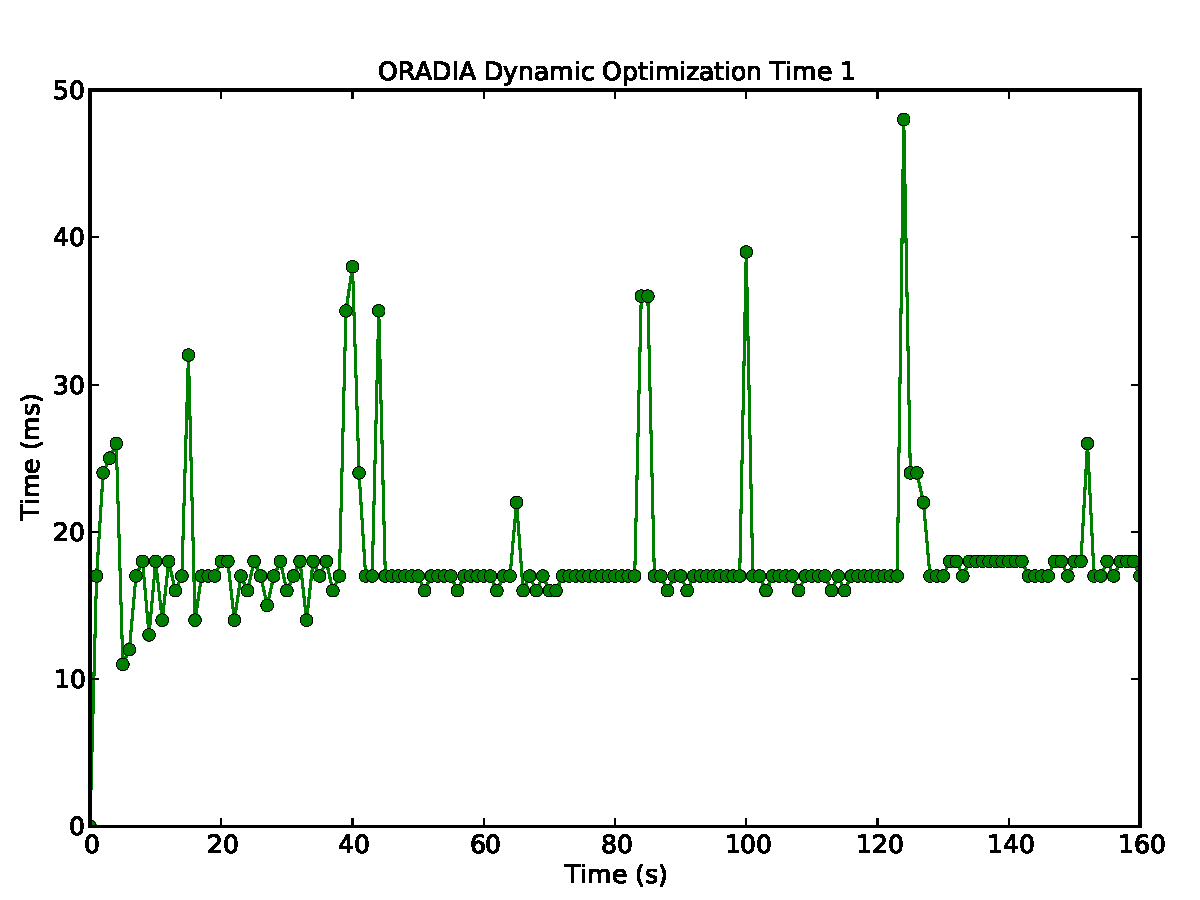
\includegraphics[bb=0 0 576 432,width=\columnwidth]{opt_time.pdf}
%		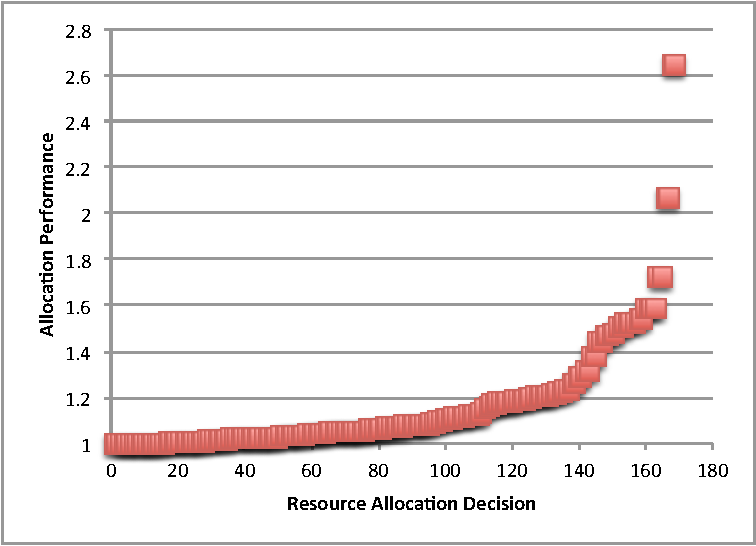
\includegraphics[width=.45\textwidth]{parsec_decision_points.pdf}
		\caption{Performance of our penalty optimization algorithm}
		\label{optimization_perf}
	\end{center}
\end{figure}

Figure~\ref{optimization_perf} shows performance of penalty optimization algorithm implemented in \tess.  

%For our video conferencing scenario the average runtime is \fix{x} and then worst case runtime is \fix{y}.  \fix{explain where the variance comes from}
